% Niveau :      PCSI *
% Discipline :  Méca
% Mots clés :   Trajectoire particule chargée

\begin{exercise}{Iridescence d'une flaque d'huile}{3}{Spé}
{Optique ondulatoire, Fabry-Pérot,Réseau de Bragg}{bermu}

\begin{questions}
\questioncours Interférence à 2 ondes.

\begin{EnvUplevel}
\begin{figure}[H]
    \centering
    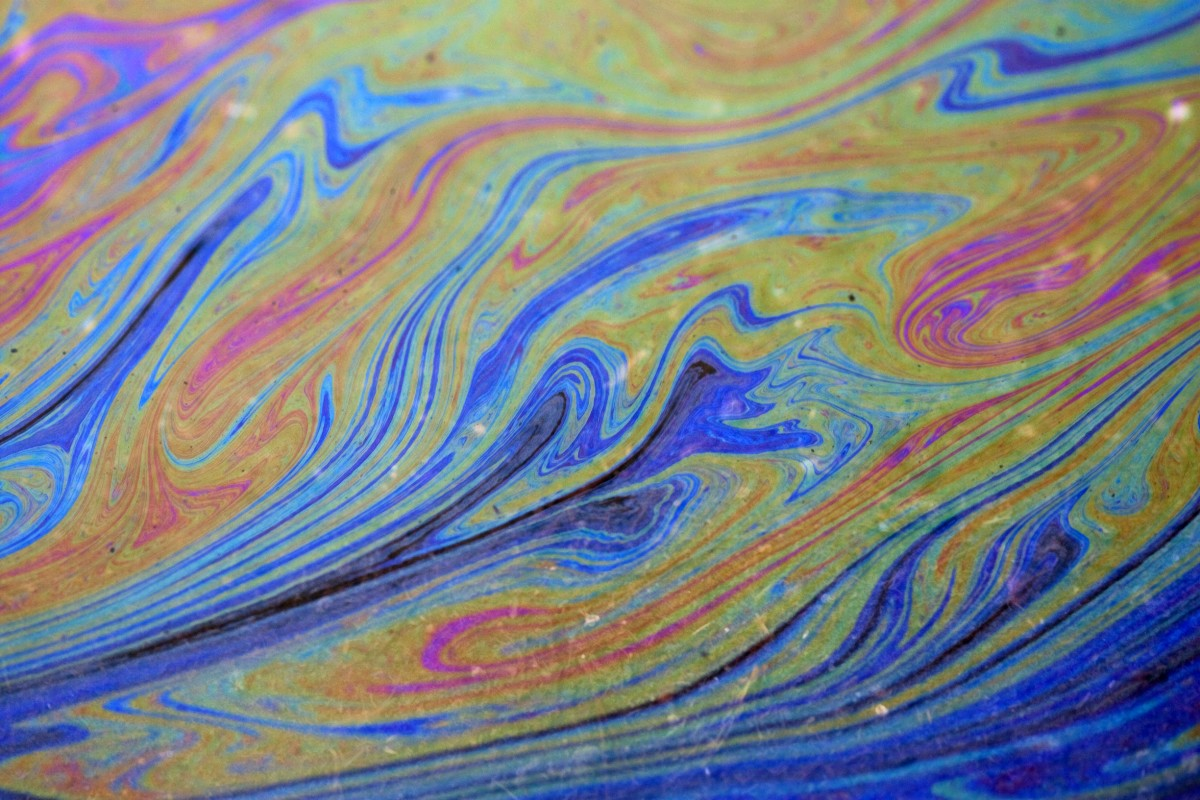
\includegraphics[width=.8\linewidth]{optique/interferences/iridescence.png}
    \caption{Irisations dans une flaque d'huile.}
    \label{fig:my_label}
\end{figure}

Nous allons à présent essayer de comprendre ce qui cause le phénomène d'iridescence lorsqu'il y a une tache d'huile sur une surface. On modélise pour cela la tache comme une couche d'huile d'épaisseur $e$ et d'indice $n = 1.5$ en surface du sol et surmontée d'air, d'indice 1. Un rayon lumineux de longueur d'onde $\lambda$ et d'intensité $I_0$ arrive sous incidence $\theta_1$.

Il est réfléchi/transmis de multiples fois. Le coefficient de réflexion en amplitude air/huile est noté $r$ et celui de transmission $t$. On considère que la réflexion est totale sur l'interface huile/sol.
\end{EnvUplevel}

\question Faire un schéma du modèle illustrant les réflexions multiples. Expliquer qualitativement le principe et où se formeront les interférences.

\question Quel est la différence de marche $\delta$ entre deux ondes réfléchies consécutives ? En quoi peut-on qualifier ce dispositif de réseau ?

\question Montrez que l'amplitude totale peut se mettre sous la forme suivante
$$A = A_0 \dfrac{r + (t^2-r^2) e^{i 2\pi\frac{\delta}{\lambda}}}{1 - r e^{i 2\pi\frac{\delta}{\lambda}}}.$$

\question En déduire la forme suivante pour l'amplitude
$$I = I_0\cal{F} \dfrac{\frac{(r+t^2-r^2)^2}{4r} + (t^2-r^2) \sin^2\qty(\pi\frac{\delta}{\lambda})}{1 + \cal{F} \sin^2\qty(\pi\frac{\delta}{\lambda})},$$
avec $\cal{F}$, la finesse de l'interféromètre dont on pourra donner l'expression et une interprétation physique.

\uplevel{Pour une onde polarisée correctement$^\dagger$, les coefficients de réflexion en amplitude sont
$$r = \dfrac{\cos\theta_1 - n \cos\theta_2}{ \cos\theta_1 + n \cos\theta_2}, \qquad t = 1 + r,$$
avec $\theta_2$ l'angle de réfraction dans l'huile.}

\question Comment ce simplifie cette expression sous incidence quasi-normale ? Tracer le profil $I(x = \delta/\lambda)$. Interpréter ces résultats au vue de la figure ci-dessus.
\end{questions}

$^\dagger$ {\small Polarisation dite transverse électronique ou s.}
\end{exercise} 

\begin{solution}


\begin{questions}
\questioncours Interférence à 2 ondes.

\question À l'infini : il faut être loin (devant $e$), ou mettre une lentille.

\question $\delta = 2ne \cos\theta_1$, au moins aux petits angles...

\question On somme, bien faire attention à ne pas faire la récurrence trop vite

\question  $\cal{F} = \frac{4r}{1-r^2}$ (comme pour un FP normal), rend compte de la selectivite du dispositif

\uplevel{Pour une onde polarisée correctement$^\dagger$, les coefficients de réflexion en amplitude sont
$$r = \dfrac{\cos\theta_1 - n \cos\theta_2}{ \cos\theta_1 + n \cos\theta_2}, \qquad t = 1 + r,$$
et le coefficient en intensité $R = \abs{r}^2$.}

\question Inicidence quasi normale: $\theta_1\approx\theta_2\approx 0$ i.e. $r\approx \frac{1-n}{1+n}$. La fonction d'airy a des pics très piqués : Si on change nu peu de lambda, on change un peu où on a des interf constructives. Faire dire que l'epaisseur de la lame d'huile doit etre d'ordre de $\lambda$ sinon ça ne marche pas.
\end{questions}

\end{solution}